% Generated by Sphinx.
\def\sphinxdocclass{report}
\documentclass[letterpaper,10pt,english]{sphinxmanual}
\usepackage[utf8]{inputenc}
\DeclareUnicodeCharacter{00A0}{\nobreakspace}
\usepackage{cmap}
\usepackage[T1]{fontenc}
\usepackage[french]{babel}
\usepackage{times}
\usepackage[Bjarne]{fncychap}
\usepackage{longtable}
\usepackage{sphinx}
\usepackage{multirow}


\title{Documentation Onitu}
\date{16 mars 2014}
\release{0.1-prev}
\author{Yannick PÉROUX, Alexandre Baron, Antoine Rozo, Wannes Rombouts, Louis Roche, Maxime Constantinian, Morgan Faget, Mathis Dupuy}
\newcommand{\sphinxlogo}{}
\renewcommand{\releasename}{Release}
\makeindex

\makeatletter
\def\PYG@reset{\let\PYG@it=\relax \let\PYG@bf=\relax%
    \let\PYG@ul=\relax \let\PYG@tc=\relax%
    \let\PYG@bc=\relax \let\PYG@ff=\relax}
\def\PYG@tok#1{\csname PYG@tok@#1\endcsname}
\def\PYG@toks#1+{\ifx\relax#1\empty\else%
    \PYG@tok{#1}\expandafter\PYG@toks\fi}
\def\PYG@do#1{\PYG@bc{\PYG@tc{\PYG@ul{%
    \PYG@it{\PYG@bf{\PYG@ff{#1}}}}}}}
\def\PYG#1#2{\PYG@reset\PYG@toks#1+\relax+\PYG@do{#2}}

\expandafter\def\csname PYG@tok@gd\endcsname{\def\PYG@tc##1{\textcolor[rgb]{0.63,0.00,0.00}{##1}}}
\expandafter\def\csname PYG@tok@gu\endcsname{\let\PYG@bf=\textbf\def\PYG@tc##1{\textcolor[rgb]{0.50,0.00,0.50}{##1}}}
\expandafter\def\csname PYG@tok@gt\endcsname{\def\PYG@tc##1{\textcolor[rgb]{0.00,0.27,0.87}{##1}}}
\expandafter\def\csname PYG@tok@gs\endcsname{\let\PYG@bf=\textbf}
\expandafter\def\csname PYG@tok@gr\endcsname{\def\PYG@tc##1{\textcolor[rgb]{1.00,0.00,0.00}{##1}}}
\expandafter\def\csname PYG@tok@cm\endcsname{\let\PYG@it=\textit\def\PYG@tc##1{\textcolor[rgb]{0.25,0.50,0.56}{##1}}}
\expandafter\def\csname PYG@tok@vg\endcsname{\def\PYG@tc##1{\textcolor[rgb]{0.73,0.38,0.84}{##1}}}
\expandafter\def\csname PYG@tok@m\endcsname{\def\PYG@tc##1{\textcolor[rgb]{0.13,0.50,0.31}{##1}}}
\expandafter\def\csname PYG@tok@mh\endcsname{\def\PYG@tc##1{\textcolor[rgb]{0.13,0.50,0.31}{##1}}}
\expandafter\def\csname PYG@tok@cs\endcsname{\def\PYG@tc##1{\textcolor[rgb]{0.25,0.50,0.56}{##1}}\def\PYG@bc##1{\setlength{\fboxsep}{0pt}\colorbox[rgb]{1.00,0.94,0.94}{\strut ##1}}}
\expandafter\def\csname PYG@tok@ge\endcsname{\let\PYG@it=\textit}
\expandafter\def\csname PYG@tok@vc\endcsname{\def\PYG@tc##1{\textcolor[rgb]{0.73,0.38,0.84}{##1}}}
\expandafter\def\csname PYG@tok@il\endcsname{\def\PYG@tc##1{\textcolor[rgb]{0.13,0.50,0.31}{##1}}}
\expandafter\def\csname PYG@tok@go\endcsname{\def\PYG@tc##1{\textcolor[rgb]{0.20,0.20,0.20}{##1}}}
\expandafter\def\csname PYG@tok@cp\endcsname{\def\PYG@tc##1{\textcolor[rgb]{0.00,0.44,0.13}{##1}}}
\expandafter\def\csname PYG@tok@gi\endcsname{\def\PYG@tc##1{\textcolor[rgb]{0.00,0.63,0.00}{##1}}}
\expandafter\def\csname PYG@tok@gh\endcsname{\let\PYG@bf=\textbf\def\PYG@tc##1{\textcolor[rgb]{0.00,0.00,0.50}{##1}}}
\expandafter\def\csname PYG@tok@ni\endcsname{\let\PYG@bf=\textbf\def\PYG@tc##1{\textcolor[rgb]{0.84,0.33,0.22}{##1}}}
\expandafter\def\csname PYG@tok@nl\endcsname{\let\PYG@bf=\textbf\def\PYG@tc##1{\textcolor[rgb]{0.00,0.13,0.44}{##1}}}
\expandafter\def\csname PYG@tok@nn\endcsname{\let\PYG@bf=\textbf\def\PYG@tc##1{\textcolor[rgb]{0.05,0.52,0.71}{##1}}}
\expandafter\def\csname PYG@tok@no\endcsname{\def\PYG@tc##1{\textcolor[rgb]{0.38,0.68,0.84}{##1}}}
\expandafter\def\csname PYG@tok@na\endcsname{\def\PYG@tc##1{\textcolor[rgb]{0.25,0.44,0.63}{##1}}}
\expandafter\def\csname PYG@tok@nb\endcsname{\def\PYG@tc##1{\textcolor[rgb]{0.00,0.44,0.13}{##1}}}
\expandafter\def\csname PYG@tok@nc\endcsname{\let\PYG@bf=\textbf\def\PYG@tc##1{\textcolor[rgb]{0.05,0.52,0.71}{##1}}}
\expandafter\def\csname PYG@tok@nd\endcsname{\let\PYG@bf=\textbf\def\PYG@tc##1{\textcolor[rgb]{0.33,0.33,0.33}{##1}}}
\expandafter\def\csname PYG@tok@ne\endcsname{\def\PYG@tc##1{\textcolor[rgb]{0.00,0.44,0.13}{##1}}}
\expandafter\def\csname PYG@tok@nf\endcsname{\def\PYG@tc##1{\textcolor[rgb]{0.02,0.16,0.49}{##1}}}
\expandafter\def\csname PYG@tok@si\endcsname{\let\PYG@it=\textit\def\PYG@tc##1{\textcolor[rgb]{0.44,0.63,0.82}{##1}}}
\expandafter\def\csname PYG@tok@s2\endcsname{\def\PYG@tc##1{\textcolor[rgb]{0.25,0.44,0.63}{##1}}}
\expandafter\def\csname PYG@tok@vi\endcsname{\def\PYG@tc##1{\textcolor[rgb]{0.73,0.38,0.84}{##1}}}
\expandafter\def\csname PYG@tok@nt\endcsname{\let\PYG@bf=\textbf\def\PYG@tc##1{\textcolor[rgb]{0.02,0.16,0.45}{##1}}}
\expandafter\def\csname PYG@tok@nv\endcsname{\def\PYG@tc##1{\textcolor[rgb]{0.73,0.38,0.84}{##1}}}
\expandafter\def\csname PYG@tok@s1\endcsname{\def\PYG@tc##1{\textcolor[rgb]{0.25,0.44,0.63}{##1}}}
\expandafter\def\csname PYG@tok@gp\endcsname{\let\PYG@bf=\textbf\def\PYG@tc##1{\textcolor[rgb]{0.78,0.36,0.04}{##1}}}
\expandafter\def\csname PYG@tok@sh\endcsname{\def\PYG@tc##1{\textcolor[rgb]{0.25,0.44,0.63}{##1}}}
\expandafter\def\csname PYG@tok@ow\endcsname{\let\PYG@bf=\textbf\def\PYG@tc##1{\textcolor[rgb]{0.00,0.44,0.13}{##1}}}
\expandafter\def\csname PYG@tok@sx\endcsname{\def\PYG@tc##1{\textcolor[rgb]{0.78,0.36,0.04}{##1}}}
\expandafter\def\csname PYG@tok@bp\endcsname{\def\PYG@tc##1{\textcolor[rgb]{0.00,0.44,0.13}{##1}}}
\expandafter\def\csname PYG@tok@c1\endcsname{\let\PYG@it=\textit\def\PYG@tc##1{\textcolor[rgb]{0.25,0.50,0.56}{##1}}}
\expandafter\def\csname PYG@tok@kc\endcsname{\let\PYG@bf=\textbf\def\PYG@tc##1{\textcolor[rgb]{0.00,0.44,0.13}{##1}}}
\expandafter\def\csname PYG@tok@c\endcsname{\let\PYG@it=\textit\def\PYG@tc##1{\textcolor[rgb]{0.25,0.50,0.56}{##1}}}
\expandafter\def\csname PYG@tok@mf\endcsname{\def\PYG@tc##1{\textcolor[rgb]{0.13,0.50,0.31}{##1}}}
\expandafter\def\csname PYG@tok@err\endcsname{\def\PYG@bc##1{\setlength{\fboxsep}{0pt}\fcolorbox[rgb]{1.00,0.00,0.00}{1,1,1}{\strut ##1}}}
\expandafter\def\csname PYG@tok@kd\endcsname{\let\PYG@bf=\textbf\def\PYG@tc##1{\textcolor[rgb]{0.00,0.44,0.13}{##1}}}
\expandafter\def\csname PYG@tok@ss\endcsname{\def\PYG@tc##1{\textcolor[rgb]{0.32,0.47,0.09}{##1}}}
\expandafter\def\csname PYG@tok@sr\endcsname{\def\PYG@tc##1{\textcolor[rgb]{0.14,0.33,0.53}{##1}}}
\expandafter\def\csname PYG@tok@mo\endcsname{\def\PYG@tc##1{\textcolor[rgb]{0.13,0.50,0.31}{##1}}}
\expandafter\def\csname PYG@tok@mi\endcsname{\def\PYG@tc##1{\textcolor[rgb]{0.13,0.50,0.31}{##1}}}
\expandafter\def\csname PYG@tok@kn\endcsname{\let\PYG@bf=\textbf\def\PYG@tc##1{\textcolor[rgb]{0.00,0.44,0.13}{##1}}}
\expandafter\def\csname PYG@tok@o\endcsname{\def\PYG@tc##1{\textcolor[rgb]{0.40,0.40,0.40}{##1}}}
\expandafter\def\csname PYG@tok@kr\endcsname{\let\PYG@bf=\textbf\def\PYG@tc##1{\textcolor[rgb]{0.00,0.44,0.13}{##1}}}
\expandafter\def\csname PYG@tok@s\endcsname{\def\PYG@tc##1{\textcolor[rgb]{0.25,0.44,0.63}{##1}}}
\expandafter\def\csname PYG@tok@kp\endcsname{\def\PYG@tc##1{\textcolor[rgb]{0.00,0.44,0.13}{##1}}}
\expandafter\def\csname PYG@tok@w\endcsname{\def\PYG@tc##1{\textcolor[rgb]{0.73,0.73,0.73}{##1}}}
\expandafter\def\csname PYG@tok@kt\endcsname{\def\PYG@tc##1{\textcolor[rgb]{0.56,0.13,0.00}{##1}}}
\expandafter\def\csname PYG@tok@sc\endcsname{\def\PYG@tc##1{\textcolor[rgb]{0.25,0.44,0.63}{##1}}}
\expandafter\def\csname PYG@tok@sb\endcsname{\def\PYG@tc##1{\textcolor[rgb]{0.25,0.44,0.63}{##1}}}
\expandafter\def\csname PYG@tok@k\endcsname{\let\PYG@bf=\textbf\def\PYG@tc##1{\textcolor[rgb]{0.00,0.44,0.13}{##1}}}
\expandafter\def\csname PYG@tok@se\endcsname{\let\PYG@bf=\textbf\def\PYG@tc##1{\textcolor[rgb]{0.25,0.44,0.63}{##1}}}
\expandafter\def\csname PYG@tok@sd\endcsname{\let\PYG@it=\textit\def\PYG@tc##1{\textcolor[rgb]{0.25,0.44,0.63}{##1}}}

\def\PYGZbs{\char`\\}
\def\PYGZus{\char`\_}
\def\PYGZob{\char`\{}
\def\PYGZcb{\char`\}}
\def\PYGZca{\char`\^}
\def\PYGZam{\char`\&}
\def\PYGZlt{\char`\<}
\def\PYGZgt{\char`\>}
\def\PYGZsh{\char`\#}
\def\PYGZpc{\char`\%}
\def\PYGZdl{\char`\$}
\def\PYGZhy{\char`\-}
\def\PYGZsq{\char`\'}
\def\PYGZdq{\char`\"}
\def\PYGZti{\char`\~}
% for compatibility with earlier versions
\def\PYGZat{@}
\def\PYGZlb{[}
\def\PYGZrb{]}
\makeatother

\begin{document}

\maketitle
\tableofcontents
\phantomsection\label{index::doc}


Onitu est un outil permettant la synchronisation de fichiers entre différents services. Cette documentation contient tout ce que vous devez connaître pour commencer à explorer Onitu.

\begin{notice}{note}{Note:}
Note: Ce document est la documentation technique. Si vous souhaitez apprendre à utiliser Onitu, tournez-vous vers la \href{http://github.com/onitu/onitu}{Documentation utilisateur}.
\end{notice}


\chapter{Table des matières}
\label{index:onitu-version-technical-documentation}\label{index:content-table}\label{index:user-documentation}

\section{Premiers pas}
\label{intro:getting-started}\label{intro::doc}

\subsection{Onitu en un clin d'œil}
\label{intro:onitu-at-a-glance}
Onitu est chargé de traiter un grand nombre d'événements provenant de services variés. Il est ainsi contruit autour d'un modèle asynchrone. Chaque composant s'exécute dans un processus séparé, et la communication est assurée par des messages ZeroMQ et à l'aide d'une base de données Redis.

Afin de synchroniser les fichiers entre différents services externes, Onitu s'appuie sur un système de pilotes (\emph{drivers}). Vous trouverez plus d'informations à ce sujet dans la rubrique {\hyperref[drivers::doc]{\emph{Création d'un nouveau pilote}}}. Chaque pilote émet et reçoit des ordres depuis le {\hyperref[components:onitu.referee.Referee]{\code{Referee}}}, qui s'occupe de déterminer où les fichiers doivent être synchronisés, suivant les règles de configuration.


\subsection{Glossaire}
\label{intro:glossary}\begin{description}
\item[{\index{Driver|textbf}Pilote}] \leavevmode\phantomsection\label{intro:term-driver}
Programme chargé de la liaison entre Onitu et un service distant (SSH, Dropbox, un disque dur…). \emph{cf} {\hyperref[drivers::doc]{\emph{Créer un nouveau pilote}}}

\item[{\index{Entry|textbf}Entrée}] \leavevmode\phantomsection\label{intro:term-entry}
Un pilote configuré par l'utilisateur. Par exemple, il peut s'agir du pilote Dropbox configuré pour utiliser un conpte utilisateur spécifique. Une entrée peut être vue comme une instance de pilote.

\item[{\index{Rule|textbf}Règle}] \leavevmode\phantomsection\label{intro:term-rule}
Fait correspondre un ensemble de fichiers à un ensemble d'entrées. Utilisé dans la configuration pour séparer les fichiers.

\item[{\index{Setup|textbf}Configuration}] \leavevmode\phantomsection\label{intro:term-setup}
Fichier de configuration au format JSON, décrivant les entrées et les règles.

\item[{\index{Referee|textbf}Referee}] \leavevmode\phantomsection\label{intro:term-referee}
Reçoit les événements depuis les pilotes et transmet les fichiers entre les entrées suivant les règles de configuration. \emph{cf} {\hyperref[components:onitu.referee.Referee]{\code{Referee}}}

\item[{\index{Plug|textbf}Plug}] \leavevmode\phantomsection\label{intro:term-plug}
Une classe qui implémente les utilitaires nécessaires à un pilote pour communiquer avec Onitu. \emph{cf} {\hyperref[drivers:onitu.api.Plug]{\code{Plug}}}

\item[{\index{Handler|textbf}Gestionnaire}] \leavevmode\phantomsection\label{intro:term-handler}
Une fonction définie par un pilote, correspondant à une tâche spécifique. Cette fonction sera appelée par le {\hyperref[drivers:onitu.api.Plug]{\code{Plug}}} au moment opportun. \emph{cf} {\hyperref[drivers:handlers]{\emph{Gestionnaires}}}

\end{description}


\subsection{Architecture globale}
\label{intro:global-architecture}
Vous pouvez ici trouver une illustration de l'architecture globale d'Onitu: {\hyperref[intro:schematic]{\emph{Figure 1.1}}}.
\begin{figure}[htbp]
\centering
\capstart

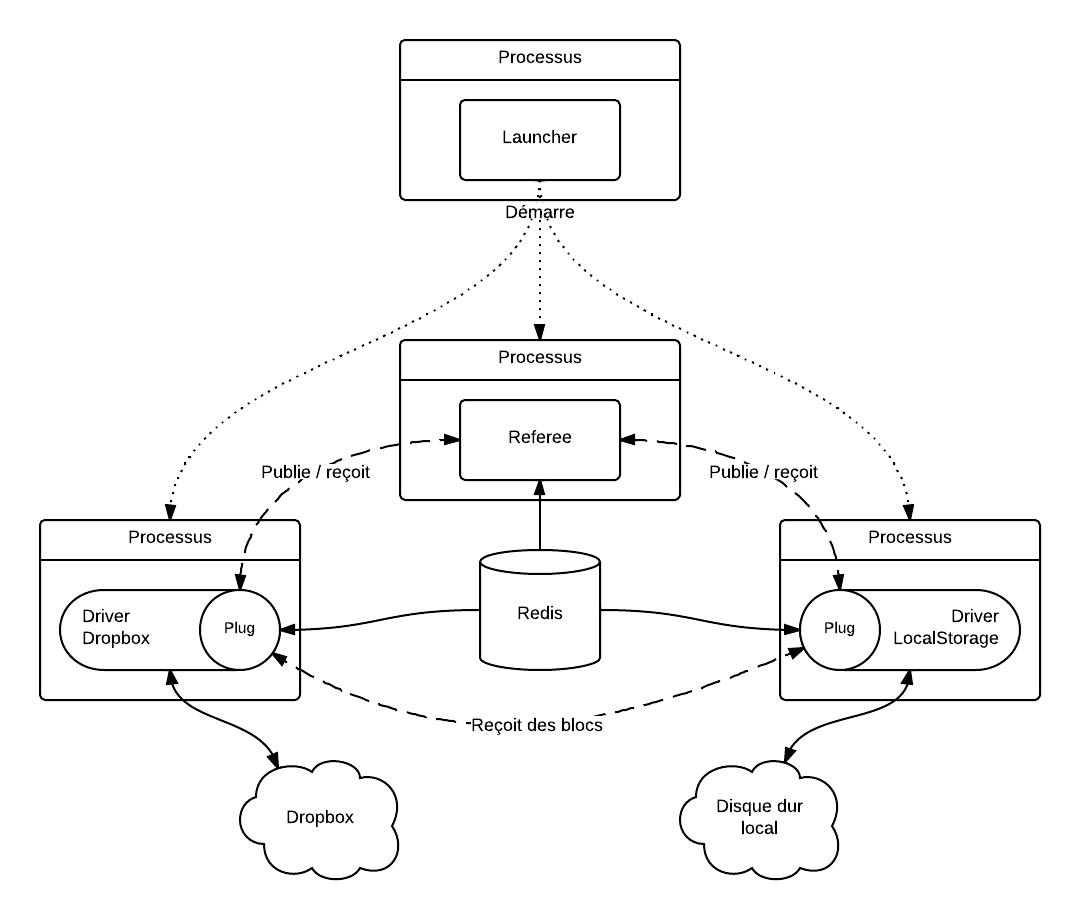
\includegraphics{global_archi.png}
\caption{Un schéma illustrant l'architecture globale d'Onitu, avec deux pilotes.}\label{intro:schematic}\end{figure}


\subsection{Dépendances}
\label{intro:dependencies}
Le cœur d'Onitu utilise différentes bibliothèques (d'autres dépendances existent mais sont spécifiques à certains pilotes):
\begin{description}
\item[{\href{http://circus.readthedocs.org}{Circus}}] \leavevmode
Utilisé pour pour le lancement, la gestion et la supervision des différents processus

\item[{\href{http://github.com/zeromq/pyzmq}{PyZMQ}}] \leavevmode
Une implémentation Python de la bibliothèque ZeroMQ

\item[{\href{http://github.com/andymccurdy/redis-py}{redis-py}}] \leavevmode
Une bibliothèque pour communiquer avec Redis depuis Python

\item[{\href{http://pythonhosted.org/Logbook/}{Logbook}}] \leavevmode
Une bibliothèque de journalisation, permettant à Onitu l'écriture sur un canal ZeroMQ, et rassemblant l'ensemble des journaux au même endroit.

\end{description}


\subsection{Choix techniques}
\label{intro:logbook}\label{intro:technical-choices}
Nous avons effectué quelques choix laborieux afin de construire Onitu dans une voie la plus efficiente et maintenable possible. Ces choix peuvent être discutables, mais en voici nos motivations:


\subsubsection{Python}
\label{intro:python}
Python est un langage polyvalent et flexible. Il fut notre premier choix, comme nous l'utilisions déjà tous et l'apprécions. Il nous permet de distribuer Onitu très facilement, sans avoir à compiler les sources ou fournir des binaires. Python est disponible sur un grand nombre de systèmes, possède de nombreuses fonctionnalités intégrées, et est simple à lire et à comprendre.

Vous avez probablement des préoccupations au niveau de la vitesse, mais Onitu est une application limitée par les entrées/sorties, une grande partie du temps d'exécution n'est pas dédiée à l'interprétation du code Python mais au téléchargement de fichiers ou à l'échange d'informations sur des \emph{sockets}. Le même programme écrit dans un langage bas-niveau tel que le C serait beaucoup plus complexe, et montrerait probablement un faible gain de performances.


\subsubsection{ZeroMQ}
\label{intro:zeromq}
Onitu étant une application se basant sur de nombreux processus et exétrons, un moyen de communicatin entre ces divers fils était nécessaire. ZeroMQ est une couche du haut du protocole IP et des \emph{sockets} Unix, et fournit des patrons de messages. Onitu en utilise plusieurs, tels ROUTER/DEALER, PUBLISH/SUBSCRIBE et REQUEST/REPLY.

ZeroMQ est très rapide, disponible sur un grand nombre de plates-formes, et possède une implémentation Python. Il est plus léger et flexible que les autres acteurs du domaine, comme RabbitMQ ou ActiveMQ.


\subsubsection{Redis}
\label{intro:redis}
Onitu nécessite l'enregistrement d'informations dans une base de données persistante. Cette base doit être multiplate-forme, sans schémas, et simple à installer et maintenir. C'est dans cette optique que nous nous sommes portés sur Redis. Cependant, Redis n'est pas disponible dans la même version sur toutes les plates-formes, et n'est pas réellement persistant. Aussi, la base de données entière est chargée en mémoire, limitant donc sa taille. Ainsi, une nouvelle solution viendra sous peu remplacer Redis, ne répondant pas parfaitement aux besoins.


\section{Création d'un nouveau pilote}
\label{drivers:creating-a-new-driver}\label{drivers::doc}
Un pilote est un programme Python permettant la synchronisation des fichiers avec un service distant, tel Dropbox, Google Drive, SSH, FTP ou un disque local.


\subsection{Bases}
\label{drivers:basics}
Les différents pilotes communiquent avec Onitu \emph{via} la classe {\hyperref[drivers:onitu.api.Plug]{\code{Plug}}}, qui traite les opérations communes à tous les pilotes. Chaque pilote implémente ses propres tâches à l'aide du système de {\hyperref[drivers:handlers]{gestionnaires}}. Ces gestionnaires seront appelés par le {\hyperref[drivers:onitu.api.Plug]{\code{Plug}}} à diverses occasions.

Les transferts de fichiers au sein d'Onitu se font par blocs. Quand un nouveau transfert débute, le {\hyperref[drivers:onitu.api.Plug]{\code{Plug}}} demande des blocs de données aux autres pilotes, et appelle ensuite le gestionnaire \emph{upload\_chunk}.

Chaque pilote doit contenir une fonction \emph{start}, prenant un nom en premier paramètre et ne retournant rien. Le nom est choisi par l'utilisateur lors de la configuration du pilote. Cette fonction est appelée par Onitu au moment de l'initialisation du pilote, et ne doit pas retourner avant la fin de vie du pilote (\emph{cf} {\hyperref[drivers:onitu.api.Plug.listen]{\code{Plug.listen()}}}).

Quand un pilote détecte la mise à jour d'un fichier, il doit actualiser les {\hyperref[drivers:onitu.api.metadata.Metadata]{\code{Metadata}}} du fichier, en spécifiant une {\hyperref[drivers:onitu.api.metadata.Metadata.revision]{\code{Metadata.revision}}}, et appeler :meth.{}`.Plug.update\_file{}`.

\begin{notice}{note}{Note:}
Au cours de leur mise en service, les pilotes doivent inspecter leur système de fichiers à la recherche de créations ou mises à jour de fichiers. Ils doivent aussi écouter ces changements tout au long de leur exécution. Le méchanisme utilisé pour cela est propre à chaque pilote, et ne peut donc pas être abstrait par le {\hyperref[drivers:onitu.api.Plug]{\code{Plug}}}.
\end{notice}

Onitu fournit un ensemble de {\hyperref[contribute:tests]{\emph{tests fonctionnels}}} que vous pouvez utiliser afin de vérifier que votre pilote corresponde aux exigences.


\subsection{Gestionnaires}
\label{drivers:id1}\label{drivers:handlers}
Un gestionnaire est une fonction qui sera appelée par le \emph{Plug} à diverses occasions, comme la récupération d'un bloc de données depuis un fichier ou le lancement d'un transfert. Les pilotes peuvent définir uniquement les gestionnaires dont ils ont besoin. Par exemple, un pilote n'ayant rien de spécifique à faire à l'initialisation d'un transfert n'est pas forcé d'implémenter le gestionnaire \emph{end\_upload}. Afin d'enregistrer un gestionnaire, le décorateur {\hyperref[drivers:onitu.api.Plug.handler]{\code{Plug.handler()}}} est utilisé.

\begin{notice}{warning}{Attention:}
Tous les gestionnaires \textbf{doivent être protégés contre les accès concurrentiels}. Le \emph{Plug} utilise plusieurs exétrons pour traîter les requêtes concurrentes, et chaque gestionnaire peut ainsi être appelé depuis l'un ou l'autre de ces exétrons. Le {\hyperref[drivers:onitu.api.Plug]{\code{Plug}}} en lui-même est protégé contre les accès concurrentiels.
\end{notice}

La liste des gestionnaires pouvant être définis dans l'état actuel du projet est la suivante:
\index{get\_chunk() (fonction built-in)}

\begin{fulllineitems}
\phantomsection\label{drivers:get_chunk}\pysiglinewithargsret{\bfcode{get\_chunk}}{\emph{filename}, \emph{offset}, \emph{size}}{}
Retourne un bloc de données depuis un fichier, de la taille indiquée et à partir de la position donnée.
\begin{quote}\begin{description}
\item[{Paramètres}] \leavevmode\begin{itemize}
\item {} 
\textbf{filename} (\emph{chaîne de caractères}) -- Chemin absolu du fichier

\item {} 
\textbf{offset} (\emph{entier}) -- Position à partir de laquelle récupérer le contenu

\item {} 
\textbf{size} (\emph{entier}) -- Taille maximale du bloc de données devant être retourné

\end{itemize}

\item[{Type de retour}] \leavevmode\begin{itemize}
\item {} 
chaîne d'octets

\end{itemize}

\end{description}\end{quote}

\end{fulllineitems}

\index{upload\_chunk() (fonction built-in)}

\begin{fulllineitems}
\phantomsection\label{drivers:upload_chunk}\pysiglinewithargsret{\bfcode{upload\_chunk}}{\emph{filename}, \emph{offset}, \emph{chunk}}{}
Écrit un bloc de données dans un fichier, à la position indiquée.
\begin{quote}\begin{description}
\item[{Paramètres}] \leavevmode\begin{itemize}
\item {} 
\textbf{filename} (\emph{chaîne de caractères}) -- Chemin absolu du fichier

\item {} 
\textbf{offset} (\emph{entier}) -- Position à laquelle écrire le contenu

\item {} 
\textbf{chunk} (\emph{chaîne d'octets}) -- Contenu devant être écrit dans le fichier

\end{itemize}

\end{description}\end{quote}

\end{fulllineitems}

\index{start\_upload() (fonction built-in)}

\begin{fulllineitems}
\phantomsection\label{drivers:start_upload}\pysiglinewithargsret{\bfcode{start\_upload}}{\emph{metadata}}{}
Initialise un nouveau transfert. Le gestionnaire est appelé au lancement d'un nouveau transfert.
\begin{quote}\begin{description}
\item[{Paramètres}] \leavevmode\begin{itemize}
\item {} 
\textbf{metadata} ({\hyperref[drivers:onitu.api.metadata.Metadata]{\code{Metadata}}}) -- Métadonnées du fichier transféré

\end{itemize}

\end{description}\end{quote}

\end{fulllineitems}

\index{restart\_upload() (fonction built-in)}

\begin{fulllineitems}
\phantomsection\label{drivers:restart_upload}\pysiglinewithargsret{\bfcode{restart\_upload}}{\emph{metadata}, \emph{offset}}{}
Relance un transfert défectueux. Ce gestionnaire sera appelé au lancement si un transfert a été stoppé.
\begin{quote}\begin{description}
\item[{Paramètres}] \leavevmode\begin{itemize}
\item {} 
\textbf{metadata} ({\hyperref[drivers:onitu.api.metadata.Metadata]{\code{Metadata}}}) -- Métadonnées du fichier transféré

\item {} 
\textbf{offset} (\emph{entier}) -- La position du dernier bloc envoyé

\end{itemize}

\end{description}\end{quote}

\end{fulllineitems}

\index{end\_upload() (fonction built-in)}

\begin{fulllineitems}
\phantomsection\label{drivers:end_upload}\pysiglinewithargsret{\bfcode{end\_upload}}{\emph{metadata}}{}
Appelé lorsqu'un transfert est terminé.
\begin{quote}\begin{description}
\item[{Paramètres}] \leavevmode\begin{itemize}
\item {} 
\textbf{metadata} ({\hyperref[drivers:onitu.api.metadata.Metadata]{\code{Metadata}}}) -- Métadonnées du fichier transféré

\end{itemize}

\end{description}\end{quote}

\end{fulllineitems}

\index{abort\_upload() (fonction built-in)}

\begin{fulllineitems}
\phantomsection\label{drivers:abort_upload}\pysiglinewithargsret{\bfcode{abort\_upload}}{\emph{metadata}}{}
Appelé lorsqu'un transfert est annulé. Cela peut arriver par exemple si une nouvelle version du fichier apparaît pendant le transfert.
\begin{quote}\begin{description}
\item[{Paramètres}] \leavevmode\begin{itemize}
\item {} 
\textbf{metadata} ({\hyperref[drivers:onitu.api.metadata.Metadata]{\code{Metadata}}}) -- Métadonnées du fichier transféré

\end{itemize}

\end{description}\end{quote}

\end{fulllineitems}



\subsection{Plug}
\label{drivers:the-plug}\index{Plug (classe de onitu.api)}

\begin{fulllineitems}
\phantomsection\label{drivers:onitu.api.Plug}\pysigline{\strong{class }\code{onitu.api.}\bfcode{Plug}}
Le \emph{Plug} est la méthode privilégiée pour un pilote de communiquer avec un autre pilote, le {\hyperref[components:onitu.referee.Referee]{\code{Referee}}} ou la base de données.

Chaque pilote doit instancier un nouveau \emph{Plug} et en définir les gestionnaires (voir {\hyperref[drivers:onitu.api.Plug.handler]{\code{handler()}}}).

{\hyperref[drivers:onitu.api.Plug.initialize]{\code{initialize()}}} doit être appelée au début de la fonction \emph{start}. Une fois que le pilote est prêt à recevoir des requêtes depuis les autres pilotes, il doit appeler {\hyperref[components:onitu.referee.Referee.listen]{\code{listen()}}}. Cette fonction bloque jusqu'à ce que le pilote soit fermé.
\index{get\_metadata() (méthode de onitu.api.Plug)}

\begin{fulllineitems}
\phantomsection\label{drivers:onitu.api.Plug.get_metadata}\pysiglinewithargsret{\bfcode{get\_metadata}}{\emph{filename}}{}~\begin{quote}\begin{description}
\item[{Paramètres}] \leavevmode\begin{itemize}
\item {} 
\textbf{filename} -- Le nom du fichier, avec son chemin absolu depuis la racine du pilote

\end{itemize}

\item[{Type de retour}] \leavevmode\begin{itemize}
\item {} 
{\hyperref[drivers:onitu.api.metadata.Metadata]{\code{Metadata}}}

\end{itemize}

\end{description}\end{quote}

Si le fichier n'existe pas dans Onitu, il sera créé lors de l'appel à {\hyperref[drivers:onitu.api.metadata.Metadata.write]{\code{Metadata.write()}}}.

\end{fulllineitems}

\index{handler() (méthode de onitu.api.Plug)}

\begin{fulllineitems}
\phantomsection\label{drivers:onitu.api.Plug.handler}\pysiglinewithargsret{\bfcode{handler}}{\emph{task=None}}{}
Décorateur utilisé pour enregistrer un gestionnaire pour une tâche particulière.
\begin{quote}\begin{description}
\item[{Paramètres}] \leavevmode\begin{itemize}
\item {} 
\textbf{task} (\emph{chaîne de caractères}) -- Optionnel. Nom du gestionnaire. Si non spécifié, le nom de la fonction sera utilisé.

\end{itemize}

\end{description}\end{quote}

Exemple:

\begin{Verbatim}[commandchars=\\\{\}]
\PYG{n+nd}{@plug.handler}\PYG{p}{(}\PYG{p}{)}
\PYG{k}{def} \PYG{n+nf}{get\PYGZus{}chunk}\PYG{p}{(}\PYG{n}{filename}\PYG{p}{,} \PYG{n}{offset}\PYG{p}{,} \PYG{n}{size}\PYG{p}{)}\PYG{p}{:}
    \PYG{k}{with} \PYG{n+nb}{open}\PYG{p}{(}\PYG{n}{filename}\PYG{p}{,} \PYG{l+s}{\PYGZsq{}}\PYG{l+s}{rb}\PYG{l+s}{\PYGZsq{}}\PYG{p}{)} \PYG{k}{as} \PYG{n}{f}\PYG{p}{:}
        \PYG{n}{f}\PYG{o}{.}\PYG{n}{seek}\PYG{p}{(}\PYG{n}{offset}\PYG{p}{)}
        \PYG{k}{return} \PYG{n}{f}\PYG{o}{.}\PYG{n}{read}\PYG{p}{(}\PYG{n}{size}\PYG{p}{)}
\end{Verbatim}

\end{fulllineitems}

\index{initialize() (méthode de onitu.api.Plug)}

\begin{fulllineitems}
\phantomsection\label{drivers:onitu.api.Plug.initialize}\pysiglinewithargsret{\bfcode{initialize}}{\emph{name}}{}
Initialise les différents composants du \emph{Plug}. Le pilote doit l'appeler au début de la fonction \emph{start}.
\begin{quote}\begin{description}
\item[{Paramètres}] \leavevmode\begin{itemize}
\item {} 
\textbf{name} (\emph{chaîne de caractères}) -- Nom de l'entrée courante, comme donné à la fonction \emph{start}.

\end{itemize}

\end{description}\end{quote}

\end{fulllineitems}

\index{listen() (méthode de onitu.api.Plug)}

\begin{fulllineitems}
\phantomsection\label{drivers:onitu.api.Plug.listen}\pysiglinewithargsret{\bfcode{listen}}{\emph{wait=True}}{}
Lance l'écoute des requêtes en provenance des autres pilotes ou du
{\hyperref[components:onitu.referee.Referee]{\code{Referee}}}.
\begin{quote}\begin{description}
\item[{Paramètres}] \leavevmode\begin{itemize}
\item {} 
\textbf{wait} (\emph{booléen}) -- Optionnel. Si \emph{True}, bloque jusqu'à ce que le \emph{Plug} se termine. Par défaut à \emph{True}.

\end{itemize}

\end{description}\end{quote}

Cette méthode lance deux exétrons:
\begin{itemize}
\item {} \index{Plug.Router (classe de onitu.api.router)}

\begin{fulllineitems}
\phantomsection\label{drivers:onitu.api.router.Plug.Router}\pysiglinewithargsret{\strong{class }\bfcode{Router}}{\emph{plug}}{}
Reçoit et répond aux requêtes provenant des autres pilotes. C'est ce composant qui appelle le gestionnaire \emph{get\_chunk}. Il utilise un seul fil d'exécution, ce qui signifie qu'une seul appel à \emph{get\_chunk} peut être réalisé simultanément.

\end{fulllineitems}


\item {} \index{Dealer (classe de onitu.api.dealer)}

\begin{fulllineitems}
\phantomsection\label{drivers:onitu.api.dealer.Dealer}\pysiglinewithargsret{\strong{class }\code{onitu.api.dealer.}\bfcode{Dealer}}{\emph{plug}}{}
Reçoit et répond aux ordres provenant du \emph{Referee}.

Toutes les requêtes sont traitées dans une file d'exétrons.

\end{fulllineitems}


\end{itemize}

\end{fulllineitems}

\index{update\_file() (méthode de onitu.api.Plug)}

\begin{fulllineitems}
\phantomsection\label{drivers:onitu.api.Plug.update_file}\pysiglinewithargsret{\code{Plug.}\bfcode{update\_file}}{\emph{metadata}}{}
Cette méthode doit être appelée par le pilote après chaque création ou mise à jour de fichier. Elle prend en paramètre un objet {\hyperref[drivers:onitu.api.metadata.Metadata]{\code{Metadata}}} contenant les nouvelles valeurs des propriétés du fichier.

\end{fulllineitems}


\end{fulllineitems}



\subsection{Metadata}
\label{drivers:metadata}\index{Metadata (classe de onitu.api.metadata)}

\begin{fulllineitems}
\phantomsection\label{drivers:onitu.api.metadata.Metadata}\pysiglinewithargsret{\strong{class }\code{onitu.api.metadata.}\bfcode{Metadata}}{\emph{plug=None}, \emph{filename=None}, \emph{size=0}}{}
Cette classe représente les métadonnées de tout fichier au sein d'Onitu.

Elle doit toujours être instanciée à l'aide des méthodes de classe {\hyperref[drivers:onitu.api.metadata.Metadata.get_by_id]{\code{get\_by\_id()}}} ou {\hyperref[drivers:onitu.api.metadata.Metadata.get_by_filename]{\code{get\_by\_filename()}}}. Cependant, les pilotes ne doivent jamais instancier de nouveaux objets {\hyperref[drivers:onitu.api.metadata.Metadata]{\code{Metadata}}} d'eux-mêmes, mais utiliser la fonction {\hyperref[drivers:onitu.api.Plug.get_metadata]{\code{Plug.get\_metadata()}}}.

Les attributs possibles pour chaque fichier sont les suivants:
\begin{description}
\item[{\textbf{filename}}] \leavevmode-
Le chemin absolu vers le fichier.

\item[{\textbf{size}}] \leavevmode-
La taille du fichier, en octets.

\item[{\textbf{revision}}] \leavevmode-
Ce champ est spécifique à chaque entrée. C'est une chaîne de caractères représentant la version actuelle du fichier pour cette entrée. Le pilote se sert de ce champ pour comparer une version locale avec une version distante. Le format est dépendant du pilote (il peut être ce que vous souhaitez: un \emph{timestamp}, un nombre, un \emph{hash}…).

\item[{\textbf{owners}}] \leavevmode-
La liste des entrées possédant ce fichier.

\item[{\textbf{uptodate}}] \leavevmode-
La liste des entrées possédant une version à jour de ce fichier.

\end{description}
\index{get\_by\_filename() (méthode de classe onitu.api.metadata.Metadata)}

\begin{fulllineitems}
\phantomsection\label{drivers:onitu.api.metadata.Metadata.get_by_filename}\pysiglinewithargsret{\strong{classmethod }\bfcode{get\_by\_filename}}{\emph{plug}, \emph{filename}}{}
Instancie un nouvel objet {\hyperref[drivers:onitu.api.metadata.Metadata]{\code{Metadata}}} depuis le nom de fichier donné en paramètre.

\end{fulllineitems}

\index{get\_by\_id() (méthode de classe onitu.api.metadata.Metadata)}

\begin{fulllineitems}
\phantomsection\label{drivers:onitu.api.metadata.Metadata.get_by_id}\pysiglinewithargsret{\strong{classmethod }\bfcode{get\_by\_id}}{\emph{plug}, \emph{fid}}{}
Instancie un nouvel objet {\hyperref[drivers:onitu.api.metadata.Metadata]{\code{Metadata}}} depuis l'identifiant de fichier donné en paramètre.

\end{fulllineitems}

\index{write() (méthode de onitu.api.metadata.Metadata)}

\begin{fulllineitems}
\phantomsection\label{drivers:onitu.api.metadata.Metadata.write}\pysiglinewithargsret{\bfcode{write}}{}{}
Écrit en base les métadonnées du fichier courant.

\end{fulllineitems}

\index{write\_revision() (méthode de onitu.api.metadata.Metadata)}

\begin{fulllineitems}
\phantomsection\label{drivers:onitu.api.metadata.Metadata.write_revision}\pysiglinewithargsret{\bfcode{write\_revision}}{}{}
Écrit en base la révision actuelle du fichier. Appelée par {\hyperref[drivers:onitu.api.metadata.Metadata.write]{\code{write()}}}.

\end{fulllineitems}


\end{fulllineitems}



\subsection{Exemple}
\label{drivers:example}
Généralement, les pilotes sont créés sous la forme d'un ensemble de fonctions dans un même fichier, avec une variable globale pour le \emph{Plug}. Cependant, vous pouvez utiliser un autre style à votre convenance, comme une classe par exemple.

Vous trouverez ci-dessous l'exemple d'un simple pilote gérant le système de fichiers local:

\begin{Verbatim}[commandchars=\\\{\},numbers=left,firstnumber=1,stepnumber=1]
\PYG{k+kn}{import} \PYG{n+nn}{os}

\PYG{k+kn}{from} \PYG{n+nn}{onitu.api} \PYG{k+kn}{import} \PYG{n}{Plug}

\PYG{c}{\PYGZsh{} Une bibliothèque factice supposée surveiller le système de fichiers}
\PYG{k+kn}{from} \PYG{n+nn}{fsmonitor} \PYG{k+kn}{import} \PYG{n}{FSWatcher}

\PYG{n}{plug} \PYG{o}{=} \PYG{n}{Plug}\PYG{p}{(}\PYG{p}{)}


\PYG{n+nd}{@plug.handler}\PYG{p}{(}\PYG{p}{)}
\PYG{k}{def} \PYG{n+nf}{get\PYGZus{}chunk}\PYG{p}{(}\PYG{n}{filename}\PYG{p}{,} \PYG{n}{offset}\PYG{p}{,} \PYG{n}{size}\PYG{p}{)}\PYG{p}{:}
    \PYG{k}{with} \PYG{n+nb}{open}\PYG{p}{(}\PYG{n}{filename}\PYG{p}{,} \PYG{l+s}{\PYGZsq{}}\PYG{l+s}{rb}\PYG{l+s}{\PYGZsq{}}\PYG{p}{)} \PYG{k}{as} \PYG{n}{f}\PYG{p}{:}
        \PYG{n}{f}\PYG{o}{.}\PYG{n}{seek}\PYG{p}{(}\PYG{n}{offset}\PYG{p}{)}
        \PYG{k}{return} \PYG{n}{f}\PYG{o}{.}\PYG{n}{read}\PYG{p}{(}\PYG{n}{size}\PYG{p}{)}


\PYG{n+nd}{@plug.handler}\PYG{p}{(}\PYG{p}{)}
\PYG{k}{def} \PYG{n+nf}{upload\PYGZus{}chunk}\PYG{p}{(}\PYG{n}{filename}\PYG{p}{,} \PYG{n}{offset}\PYG{p}{,} \PYG{n}{chunk}\PYG{p}{)}\PYG{p}{:}
    \PYG{k}{with} \PYG{n+nb}{open}\PYG{p}{(}\PYG{n}{filename}\PYG{p}{,} \PYG{l+s}{\PYGZsq{}}\PYG{l+s}{ab}\PYG{l+s}{\PYGZsq{}}\PYG{p}{)} \PYG{k}{as} \PYG{n}{f}\PYG{p}{:}
        \PYG{n}{f}\PYG{o}{.}\PYG{n}{seek}\PYG{p}{(}\PYG{n}{offset}\PYG{p}{)}
        \PYG{n}{f}\PYG{o}{.}\PYG{n}{write}\PYG{p}{(}\PYG{n}{chunk}\PYG{p}{)}


\PYG{n+nd}{@plug.handler}\PYG{p}{(}\PYG{p}{)}
\PYG{k}{def} \PYG{n+nf}{end\PYGZus{}upload}\PYG{p}{(}\PYG{n}{metadata}\PYG{p}{)}\PYG{p}{:}
    \PYG{n}{metadata}\PYG{o}{.}\PYG{n}{revision} \PYG{o}{=} \PYG{n}{os}\PYG{o}{.}\PYG{n}{path}\PYG{o}{.}\PYG{n}{getmtime}\PYG{p}{(}\PYG{n}{metadata}\PYG{o}{.}\PYG{n}{filename}\PYG{p}{)}
    \PYG{n}{metadata}\PYG{o}{.}\PYG{n}{write\PYGZus{}revision}\PYG{p}{(}\PYG{p}{)}


\PYG{k}{class} \PYG{n+nc}{Watcher}\PYG{p}{(}\PYG{n}{FSWatcher}\PYG{p}{)}\PYG{p}{:}
    \PYG{k}{def} \PYG{n+nf}{on\PYGZus{}update}\PYG{p}{(}\PYG{n+nb+bp}{self}\PYG{p}{,} \PYG{n}{filename}\PYG{p}{)}\PYG{p}{:}
        \PYG{l+s+sd}{\PYGZdq{}\PYGZdq{}\PYGZdq{}Appelée chaque fois qu'une mise à jour de fichier est détectée}
\PYG{l+s+sd}{        \PYGZdq{}\PYGZdq{}\PYGZdq{}}
        \PYG{n}{metadata} \PYG{o}{=} \PYG{n}{plug}\PYG{o}{.}\PYG{n}{get\PYGZus{}metadata}\PYG{p}{(}\PYG{n}{filename}\PYG{p}{)}
        \PYG{n}{metadata}\PYG{o}{.}\PYG{n}{revision} \PYG{o}{=} \PYG{n}{os}\PYG{o}{.}\PYG{n}{path}\PYG{o}{.}\PYG{n}{getmtime}\PYG{p}{(}\PYG{n}{metadata}\PYG{o}{.}\PYG{n}{filename}\PYG{p}{)}
        \PYG{n}{metadata}\PYG{o}{.}\PYG{n}{size} \PYG{o}{=} \PYG{n}{os}\PYG{o}{.}\PYG{n}{path}\PYG{o}{.}\PYG{n}{getsize}\PYG{p}{(}\PYG{n}{metadata}\PYG{o}{.}\PYG{n}{filename}\PYG{p}{)}
        \PYG{n}{plug}\PYG{o}{.}\PYG{n}{update\PYGZus{}file}\PYG{p}{(}\PYG{n}{metadata}\PYG{p}{)}

    \PYG{k}{def} \PYG{n+nf}{check\PYGZus{}changes}\PYG{p}{(}\PYG{n+nb+bp}{self}\PYG{p}{)}\PYG{p}{:}
        \PYG{l+s+sd}{\PYGZdq{}\PYGZdq{}\PYGZdq{}Vérifie les changements sur le système de fichiers depuis le dernier lancement}
\PYG{l+s+sd}{        \PYGZdq{}\PYGZdq{}\PYGZdq{}}
        \PYG{k}{for} \PYG{n}{filename} \PYG{o+ow}{in} \PYG{n+nb+bp}{self}\PYG{o}{.}\PYG{n}{files}\PYG{p}{:}
            \PYG{n}{revision} \PYG{o}{=} \PYG{n}{os}\PYG{o}{.}\PYG{n}{path}\PYG{o}{.}\PYG{n}{getmtime}\PYG{p}{(}\PYG{n}{filename}\PYG{p}{)}
            \PYG{n}{metadata} \PYG{o}{=} \PYG{n}{plug}\PYG{o}{.}\PYG{n}{get\PYGZus{}metadata}\PYG{p}{(}\PYG{n}{filename}\PYG{p}{)}

            \PYG{c}{\PYGZsh{} Si le fichier est plus récent}
            \PYG{k}{if} \PYG{n}{revision} \PYG{o}{\PYGZgt{}} \PYG{n}{metadata}\PYG{o}{.}\PYG{n}{revision}\PYG{p}{:}
                \PYG{n}{metadata}\PYG{o}{.}\PYG{n}{revision} \PYG{o}{=} \PYG{n}{os}\PYG{o}{.}\PYG{n}{path}\PYG{o}{.}\PYG{n}{getmtime}\PYG{p}{(}\PYG{n}{metadata}\PYG{o}{.}\PYG{n}{filename}\PYG{p}{)}
                \PYG{n}{metadata}\PYG{o}{.}\PYG{n}{size} \PYG{o}{=} \PYG{n}{os}\PYG{o}{.}\PYG{n}{path}\PYG{o}{.}\PYG{n}{getsize}\PYG{p}{(}\PYG{n}{metadata}\PYG{o}{.}\PYG{n}{filename}\PYG{p}{)}
                \PYG{n}{plug}\PYG{o}{.}\PYG{n}{update\PYGZus{}file}\PYG{p}{(}\PYG{n}{metadata}\PYG{p}{)}


\PYG{k}{def} \PYG{n+nf}{start}\PYG{p}{(}\PYG{o}{*}\PYG{n}{args}\PYG{p}{,} \PYG{o}{*}\PYG{o}{*}\PYG{n}{kwargs}\PYG{p}{)}\PYG{p}{:}
    \PYG{n}{plug}\PYG{o}{.}\PYG{n}{initialize}\PYG{p}{(}\PYG{o}{*}\PYG{n}{args}\PYG{p}{,} \PYG{o}{*}\PYG{o}{*}\PYG{n}{kwargs}\PYG{p}{)}

    \PYG{n}{root} \PYG{o}{=} \PYG{n}{plug}\PYG{o}{.}\PYG{n}{options}\PYG{p}{[}\PYG{l+s}{\PYGZsq{}}\PYG{l+s}{root}\PYG{l+s}{\PYGZsq{}}\PYG{p}{]}
    \PYG{n}{os}\PYG{o}{.}\PYG{n}{chdir}\PYG{p}{(}\PYG{n}{root}\PYG{p}{)}

    \PYG{n}{watcher} \PYG{o}{=} \PYG{n}{Watcher}\PYG{p}{(}\PYG{n}{root}\PYG{p}{)}
    \PYG{n}{watcher}\PYG{o}{.}\PYG{n}{check\PYGZus{}changes}\PYG{p}{(}\PYG{p}{)}
    \PYG{n}{watcher}\PYG{o}{.}\PYG{n}{start}\PYG{p}{(}\PYG{p}{)}

    \PYG{n}{plug}\PYG{o}{.}\PYG{n}{listen}\PYG{p}{(}\PYG{p}{)}
\end{Verbatim}


\section{Documentation des composants}
\label{components::doc}\label{components:components-documentation}
Ici figure la documentation des composants non couverts par les précédentes sections. Vous n'avez pas à vous occupper de cette section si vous développez un pilote, mais elle peut être très utile si vous vous intéressez au cœur d'Onitu.


\subsection{Launcher}
\label{components:launcher}\label{components:module-onitu.__main__}\index{onitu.\_\_main\_\_ (module)}
Ce module s'occupe du lancement d'Onitu, en réalisant les opérations suivantes:
\begin{itemize}
\item {} 
Évaluer les options de la ligne de commande

\item {} 
Configurer l'outil de journalisation

\item {} 
Analyser le fichier de configuration

\item {} 
Nettoyer la base de données

\item {} 
Lancer les différents composants à l'aide de la bibliothèque Circus

\end{itemize}
\index{get\_logs\_dispatcher() (module onitu.\_\_main\_\_)}

\begin{fulllineitems}
\phantomsection\label{components:onitu.__main__.get_logs_dispatcher}\pysiglinewithargsret{\code{onitu.\_\_main\_\_.}\bfcode{get\_logs\_dispatcher}}{\emph{uri=None}, \emph{debug=False}}{}
Configure le répartiteur qui affichera les journaux reçus sur le canal ZeroMQ.

\end{fulllineitems}

\index{start\_setup() (module onitu.\_\_main\_\_)}

\begin{fulllineitems}
\phantomsection\label{components:onitu.__main__.start_setup}\pysiglinewithargsret{\code{onitu.\_\_main\_\_.}\bfcode{start\_setup}}{\emph{*args}, \emph{**kwargs}}{}
Analyse un fichier de configuration JSON, nettoie la base de données, démarre le {\hyperref[components:onitu.referee.Referee]{\code{Referee}}} et les pilotes.

\end{fulllineitems}

\index{start\_watcher() (module onitu.\_\_main\_\_)}

\begin{fulllineitems}
\phantomsection\label{components:onitu.__main__.start_watcher}\pysiglinewithargsret{\code{onitu.\_\_main\_\_.}\bfcode{start\_watcher}}{\emph{*args}, \emph{**kwargs}}{}
Démarre un superviseur Circus. Si une commande est déjà en cours d'exécution, renouvelle l'essai.

\end{fulllineitems}



\subsection{Referee}
\label{components:referee}
Le rôle du \emph{Referee} est de recevoir les événements émis par les pilotes, et d'envoyer des notifications aux autres pilotes, en fonction des règles de configuration.
\index{Referee (classe de onitu.referee)}

\begin{fulllineitems}
\phantomsection\label{components:onitu.referee.Referee}\pysigline{\strong{class }\code{onitu.referee.}\bfcode{Referee}}
Classe arbitre, reçoit tous les événements et les traite.

Les événements sont représentés par une liste Redis `event' à laquelle ils doivent être ajoutés \emph{via} un RPUSH. Chaque élément de la liste est un identifiant de fichier (\emph{fid}) du fichier ayant déclenché l'evénement.

Le \emph{Referee} communique des ordres aux entrées à l'aide d'une \emph{socket} ZMQ PUB, dont le port est stocké dans la clef Redis `referee:publisher'. Le \emph{Plug} de chaque entrée doit souscrire à ce port \emph{via} une \emph{socket} PULL, et souscrire à tous les événements débutant par son nom.

Les notifications sont envoyées aux éditeurs sous la forme de messages multipart contenant 3 éléments:
\begin{itemize}
\item {} 
Le nom de l'\emph{addressee} (du canal)

\item {} 
Le nom de l'entrée depuis laquelle le fichier doit être transféré

\item {} 
L'identifiant du fichier

\end{itemize}
\index{listen() (méthode de onitu.referee.Referee)}

\begin{fulllineitems}
\phantomsection\label{components:onitu.referee.Referee.listen}\pysiglinewithargsret{\bfcode{listen}}{}{}
Écoute tous les événements, et les traite.

\end{fulllineitems}


\end{fulllineitems}



\subsection{Utilitaires}
\label{components:utils}\label{components:module-onitu.utils}\index{onitu.utils (module)}
Ce module fournit un ensemble de classes et de fonctions utiles dans plusieurs composants d'Onitu.
\index{Redis (classe de onitu.utils)}

\begin{fulllineitems}
\phantomsection\label{components:onitu.utils.Redis}\pysiglinewithargsret{\strong{class }\code{onitu.utils.}\bfcode{Redis}}{\emph{*args}, \emph{**kwargs}}{}
Cette classe est une simple abstraction de l'objet \code{redis.Redis} de la bibliothèque redis-py.

Elle ajoute un attribut \code{session} qui préfixera toutes les clefs de la base Redis par cette session.

Cette clef de session est utilisée par Onitu pour séparer les différentes instances en base. Redis ne gérant qu'un faible nombre de bases de données, nous utilisons une base unique, mais préfixons les clefs.

L'attribut de session doit toujours être utilisé.

\end{fulllineitems}

\index{connect\_to\_redis() (module onitu.utils)}

\begin{fulllineitems}
\phantomsection\label{components:onitu.utils.connect_to_redis}\pysiglinewithargsret{\code{onitu.utils.}\bfcode{connect\_to\_redis}}{\emph{*args}, \emph{**kwargs}}{}
Cette fonction retourne un nouvel objet {\hyperref[components:onitu.utils.Redis]{\code{Redis}}}, prêt à recevoir des requêtes, et avec une session activée. La fonction bloque jusqu'à ce que la connexion soit faite.

Vous pouvez passer des arguments supplémentaires à la classe {\hyperref[components:onitu.utils.Redis]{\code{Redis}}} en les fournissant à cette fonction.

\end{fulllineitems}



\section{Contribuer à Onitu}
\label{contribute:contributing-to-onitu}\label{contribute::doc}
Onitu est un projet ouvert, dont les sources sont disponibles sur Github, et nous serions très heureux d'intégrer des corrections ou des fonctionnalités de la part de la communauté.

Voici quelques lignes directrices dans le cas où vous vous plongeriez dans le code ou rencontriez des problèmes.


\subsection{Rapports de bogues}
\label{contribute:reporting-issues}
Quand vous rencontrez des problèmes avec Onitu, nous aimons en être informés. Non pas que nous aimions que des bogues surviennent dans Onitu, mais il est préférable de les corriger que de les laisser en place.

Si vous êtes amené à faire un rapport de bogue, pensez à inclure toutes les informations que vous avez en votre possession, voici quelques conseils pour avoir un rapport le plus pertinent possible:
\begin{itemize}
\item {} 
Si le problème est reproductible, relancez Onitu en mode de débogage.

\item {} 
Onitu journalise son exécution sur la sortie, cette sortie nous est très utile pour la compréhension du problème.

\item {} 
Tentez de simplifier le problème en ne gardant que l'ensemble minimal d'actions permettant de le reproduire.

\end{itemize}


\subsection{Lancement des tests}
\label{contribute:tests}\label{contribute:running-the-tests}
Si vous développez une nouvelle fonctionnalité ou souhaitez simplement tester votre installation d'Onitu, vous pouvez exécuter les tests unitaires.

Pour cela, vous devrez installer les dépendances nécessaires au dispositif de tests, ce qui peut facilement être réalisé par la commande \emph{pip install -r requirements\_dev.txt}.

Les tests unitaires peuvent être lancés à l'aide de la commande \emph{py.test tests/}. Vous pouvez aussi vous aider de \emph{tox} afin de générer automatiquement un environnement propre et fonctionnel pour le lancement des tests.

Enfin, quelques variables d'environnement que voici peuvent vous être utiles lors de l'exécution des tests:
\begin{quote}
\begin{description}
\item[{ONITU\_TEST\_TIME\_UNIT}] \leavevmode
Plusieurs tests se basent sur un délai d'exécution avant de considérer un transfert en échec. Cette variable contient donc un nombre de secondes correspondant à l'unité de temps, \emph{1s} par défaut.

\item[{ONITU\_TEST\_DRIVER}] \leavevmode
La batterie de tests n'est exécutée que pour un pilote à la fois, cette variable permet de déterminer quel pilote sera testé, et peut donc prendre des valeurs telles que \emph{local\_storage} ou \emph{ssh}.

\end{description}
\end{quote}


\subsection{Bonnes pratiques d'utilisation de Git}
\label{contribute:good-practices-with-git}
Afin de maintenir le projet tout en intégrant les contributions externes, nous avons besoin de mettre en place certaines règles. Ceci est d'autant plus vrai au regard de l'utilisation de Git.

Chaque développement de nouvelle fonctionnalité doit être fait dans une branche qui lui est propre. Une fois la fonctionnalité prête à être intégrée, la branche doit être rebasée sur l'état actuel de la branche \emph{develop}, avant de faire une demande de \emph{pull request}.

Les mainteneurs de la branche \emph{develop} pourront ensuite intégrer la fonctionnalité au moment venu. Ils pourraient auparavant vous demander d'effectuer quelques changements sur votre travail.

Vous ne devez jamais fusionner la branche \emph{master} sur votre branche de développement, préférez à la place rebaser votre branche.


\subsection{Style de codage}
\label{contribute:coding-style}
Vos contributions au projet doivent respecter les règles définies par la \index{Python Enhancement Proposals!PEP 008}\href{http://www.python.org/dev/peps/pep-0008}{\textbf{PEP 008}}, vous pouvez utiliser un outil tel que flake8 pour vérifier que votre code est en accord avec ces règles.

Dans le cas où vous vous poseriez la question, l'indentation utilisée est de quatre espaces.

Merci de prendre en considération ces quelques règles, qui assurent au projet de rester propre. Chaque demande de \emph{pull request} sera étudiée afin de regarder en premier lieu si le code fourni les respecte.


\section{Notes de version}
\label{changelog::doc}\label{changelog:changelog}
Vous trouverez un détail des changements entre les versions sur le \href{https://github.com/onitu/onitu/releases}{Github} du projet. Retrouvez ci-dessous un bref résumé:


\subsection{0.1}
\label{changelog:id1}
Première version

Le \emph{Referee} peut traiter de simples règles basées sur le chemin, la taille et l'extension du fichier.

Quatre pilotes sont disponibles:
\begin{itemize}
\item {} 
Fichiers locaux (\emph{Local storage})

\item {} 
Dropbox

\item {} 
Google Drive

\item {} 
SSH

\end{itemize}

La suite de tests couvre l'ensemble du \emph{Referee} et des pilotes. Quelques tests de performance sont disponibles.


\chapter{Table d'index}
\label{index:indices-and-tables}\begin{itemize}
\item {} 
\emph{genindex}

\item {} 
\emph{modindex}

\item {} 
\emph{search}

\end{itemize}


\renewcommand{\indexname}{Index des modules Python}
\begin{theindex}
\def\bigletter#1{{\Large\sffamily#1}\nopagebreak\vspace{1mm}}
\bigletter{o}
\item {\texttt{onitu.\_\_main\_\_}}, \pageref{components:module-onitu.__main__}
\item {\texttt{onitu.utils}}, \pageref{components:module-onitu.utils}
\end{theindex}

\renewcommand{\indexname}{Index}
\printindex
\end{document}
